% !TeX spellcheck = da_DK
\subsection{Software}
Patienternes data skal behandles i form af grafisk visualisering, jævnfør afsnit \ref{subsec:software} på side \pageref{subsec:software}. Derudover skal patienternes resultater i forbindelse med testen kunne gemmes til analyse og senere brug. Dette sker ved, at det analoge signal konverteres til et digitalt signal og indsendes igennem USB-isolatoren til en computer. For at imødekomme disse krav anvendes en computer med programmet MATLAB. I MATLAB designes en GUI (Graphical User Interface), hvor ved signalet fra accelerometeret visualiseres. MATLAB koden der anvendes ved optagelse af signalet er i bilag \ref{MATLAB} Signalet optages i MATLAB via NIDAQ'en. Grunden til, at der designes en GUI, er for at optimere brugervenligheden. I GUI'en ses en graf, samt fire knapper og en toolbar, dette er illustretet på \figref{Fig:GUI_generisk}. 
\begin{figure}[H] 
	\centering 
	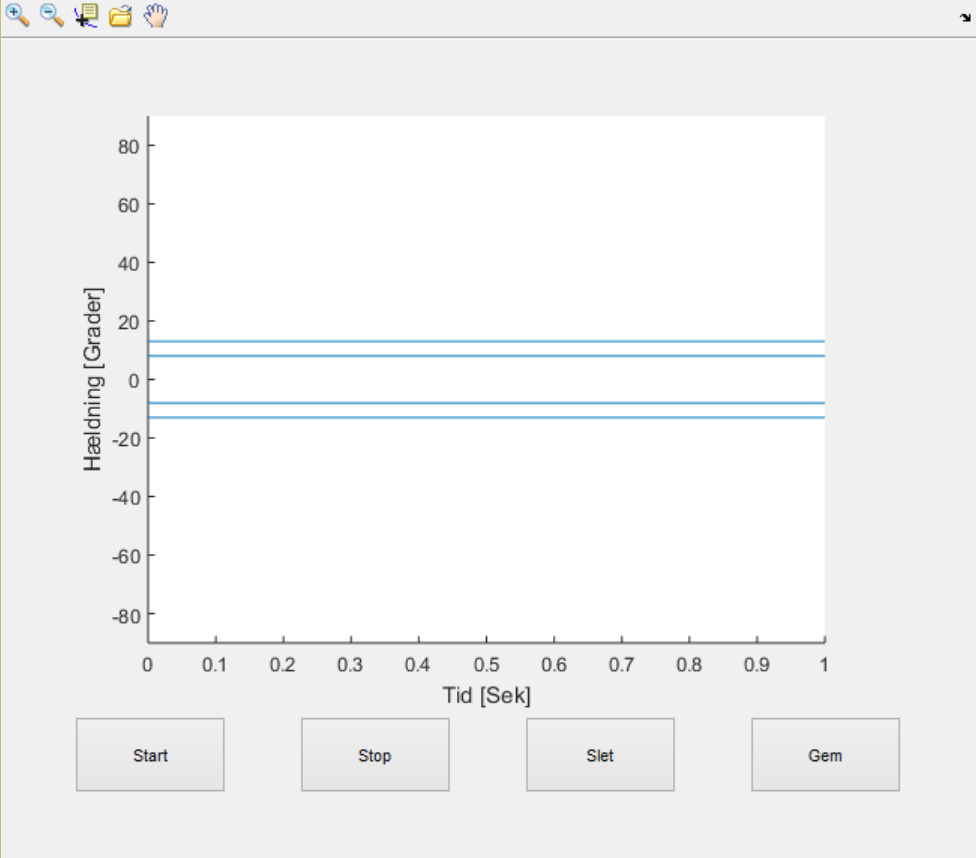
\includegraphics[scale=0.5]{figures/cProblemloesning/GUI_generisk.PNG}
	\caption{Af figuren fremgår GUI'ens display.De blå linjer illustrer de forskellige tærkselværdier i positiv og negativ retning for hhv. $\pm 8^{\circ}$ og $\pm 13^{\circ}$.}
	\label{Fig:GUI_generisk}
\end{figure} 
I koordinatsystemet måler y-aksen hældningen i grader, mens x-aksen måler tiden i sekunder. Dette gør det enkelt at se hvilken side patienten hælder til, samt i hvor lang tid patienten har befundet sig i denne position.
De fire blå linjer på tværs af koordinatsystemet er referencelinjer som illustrere de opstillede tærskelværdier for den gule og røde LED, som skal lyse i hhv. $\pm 8^{\circ}$ og $\pm 13^{\circ}$. Derved synliggøres de grænser der er for patienten, hvorved personalet herudfra kan vurdere patientens balance. I displayet er der en start-, stop-, slette- og gemmefunktion.
I toolbaren er der flere knapper, disse har til opgave at gøre det muligt at manipulere med grafen. Forstørrelsesglaset med plusset gør det muligt at zoome ind på grafen, mens forstørrelsesglaset med minusset gør det muligt at zoome ud igen. Knappen med et papir og et plus gør det muligt at aflæse det præcise punkt på grafen der markeres. Den åbne mappe gør det muligt at åbne en fil i GUI'en og hånden gør det muligt at panorere i grafen.
For at benytte GUI'en skal det fagkyndige personale følge fremgangsmåden på \ref{Fig:fremgangsmåde_software}.
\begin{figure}[H] 
	\centering 
	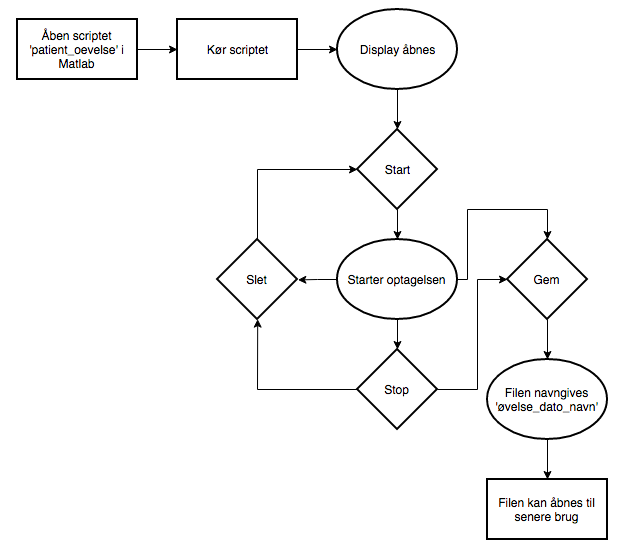
\includegraphics[scale=0.5]{figures/cProblemloesning/Software_flowdiagram.PNG}
	\caption{Flowdiagrammet viser fremgangsmåden for personalet til at benytte softwaren}
	\label{Fig:fremgangsmåde_software}
\end{figure}

\subsubsection{Test}
For at teste om softwaren viser information om patientens hældning i de bestemte tærskelværdier indsendes et input så tæt på det teoretiske som muligt. Dette gør at inputsignalet svarende til de forskellige tærskelværdier vil vise sig som hhv. $\pm 8^{\circ}$ og $\pm 13^{\circ}$ i softwarens display. Der foretages målinger for de nævnte tærskelværdier, hvorefter de enkelte optagelser gemmes.
Derudover undersøges softwaren ved at indsende en sinuskurve med en amplitude på 5.8834V og en frekvens på 500mHz, for at illustrere en svajning på \pm $90{\circ}$. Optagelsen af signalet sker ved fremgangsmåden på \ref{Fig:fremgangsmåde_software}. I forhold til det indsendte signal afviger dette fra det teoretiske input, hvilket fremgår af \ref{Tab:afvigelse_software}. Denne afvigelse er forventet da spændingen ikke er konstant og vil ændre sig over tid. 

\begin{table}[]
\centering
\caption{Af tabellen fremgår afvigelsen fra det teoretiske input til det målte input.}
\label{Tab:afvigelse_software}
\begin{tabular}{llll}
             & Teoretisk input & Målt 	& Afvigelse \\ \hline
%$2^\circ$   & 0.0670          & 0.0672  & 0.3  \% \\ \hline
%-$2^\circ$  & -0.0654         & -0.0658 & 0.6  \% \\ \hline
$8^{\circ}$   & $0.2680$          & $0.2681$  & $0.04$ \% \\ \hline
-$8^{\circ}$   & -$0.2615$         & $-0.2617$ & $0.08$ \%  \\ \hline
$13^{\circ}$  & $0.4355$          & $0.4357$  & $0.05$ \% \\ \hline
-$13^{\circ}$ & -$0.4249$         & -$0.4247$ & $0.05$ \% \\ \hline    
\end{tabular}
\end{table}

De gemte optagelserne foretaget for de forskellige tærskelværdier er illustreret på \ref{fig:software_grafer}. Det ses ud fra graferne at ved at indsende et input svarende til tærskelværdierne fås en linje som følger referenceværdierne. På figuren er der zoomet ind på de forskellige grafer, det fremgår heraf, at der kommer støj på signalet. Grunden til dette kan være at spændingen ikke er konstant og derved vil afvige under optagelsen. 
\begin{figure}[h]
\makebox[\textwidth]{%
\includegraphics[width=0.49\textwidth]{figures/cProblemloesning/(8Po.PNG}%
\hfill    
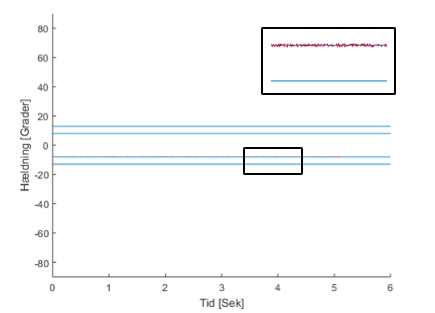
\includegraphics[width=0.49\textwidth]{figures/cProblemloesning/8Ne.PNG}%
}\\[0.5cm]% If you want some vertical space
\makebox[\textwidth]{%
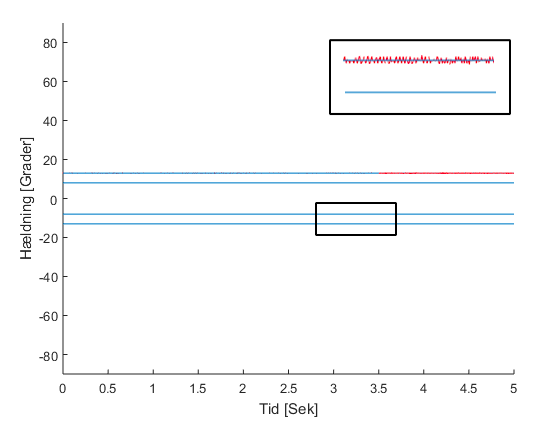
\includegraphics[width=0.49\textwidth]{figures/cProblemloesning/13Po.PNG}%
\hfill    
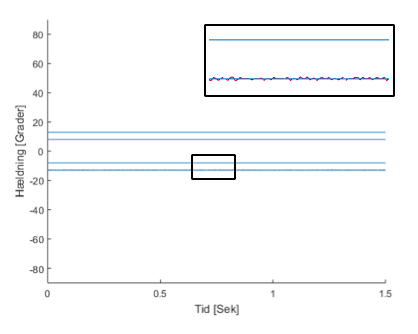
\includegraphics[width=0.49\textwidth]{figures/cProblemloesning/13Ne.PNG}%
}%
\caption{Figuren viser målingerne for de enkelte tærskelværdier. I følgende rækkefølge fra venstre mod højre: $8^{\circ}$ positiv, $8^{\circ}$ negativ, $13^{\circ}$ positiv og $13^{\circ}$ negativ.}
\label{fig:software_grafer}
\end{figure}

Det fremgår af \ref{Fig:software_sinus}, at softwaren kan visualisere en hældning fra \pm$90^{\circ}$. Ud fra dette vurderes det yderligere at softwaren kan anvendes til at visualisere kropshældning. 

\begin{figure}[H] 
	\centering 
	\includegraphics[scale=0.5]{figures/cProblemloesning/sinus.PNG}
	\caption{Figuren viser en sinuskurve som illustrere en svinging på \pm $90^{\circ}$.}
	\label{Fig:software_sinus}
\end{figure}

På baggrund af testen vurderes det at softwaren kan fremvise information om patientens hældning, derudover visualiseres det hvor meget patienten har bevæget sig ud i risikozonerne via. referencelinjer ved hhv. \pm $8^{\circ}$ og \pm $13^{\circ}$. Det er muligt at gemme dataen så denne kan anvendes senere. 





